%-------------------------------------------------------------------------------
\subsubsection{Système dynamique en $y^5$}
%-------------------------------------------------------------------------------

On s'intéresse au système dynamique gouverné par l'équation
$$
\dot y = \mu y + 2 y^3 - y^5.
$$

\begin{enumerate}
  \item Déterminer le nombre de points d'équilibre du système en fonction de $\mu$ et préciser ce ou ces points d'équilibre.
  \solution{
  On remarque que $F(y) = y(\mu + 2 y^2 - y^4)$ s'annule pour $y^* = 0$ et pour les solutions de $\{\mu + 2 y^2 - y^4 = 0\}$. \\
  En posant, $z = y^2$, $\mu + 2 z - z^2 = 0$ admet des solutions si $\Delta =  4(1 + \mu) \geq 0$, c'est-à-dire si $\mu \geq -1$. Ces solutions sont alors $z_1^* = 1 - \sqrt{1+\mu}$ et $z_2^* = 1 + \sqrt{1+\mu}$. \\
  $z_2^*$ existe et est positive pour $\mu \geq -1$. Par contre $z_1^*$ existe mais est négative (donc inadmissible puisque $z$ est un carré) quand $\mu > 0$. \\
  En notant
  $$
  y^* = 0, \qquad y_1^* = \sqrt{z_1^*}, \qquad y_2^* = \sqrt{z_2^*}
  $$
  quand ils existent. On a donc
  \begin{itemize}
    \item pour $\mu < -1$ : un unique point d'équilibre en $y_0^*$ ; 
    \item pour $\mu = -1$ : trois points d'équilibre en $y_0^*$, $y_1^* = y_2^* = 1$ et $-y_1^* = - y_2^* = -1$ ; 
    \item pour $-1 < \mu < 0$ : cinq points d'équilibre en $y_0^*$, $y_1^*$, $y_2^*$, $-y_1^*$ et $-y_2^*$;
    \item pour $\mu \geq 0$ : trois points d'équilibre en $y_0^*$, $y_2^*$ et $-y_2^*$.
  \end{itemize}
  La figure suivante donne l'évolution des points d'équilibre $y^*$ en fonction de $\mu$ :
  $$
  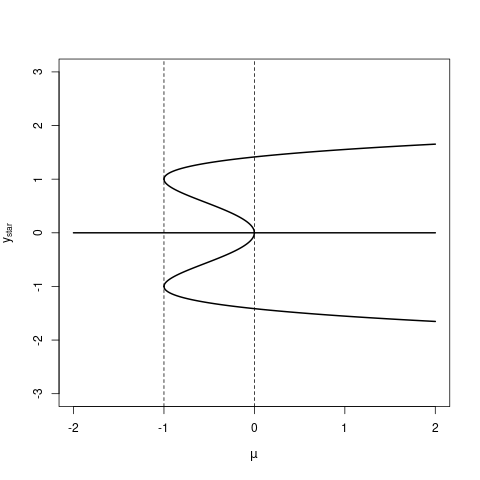
\includegraphics[width=.5\textwidth, trim=0 10 10 50, clip=]{ExoSystDynY5-yStar}
  $$
}
  %
  \item \'Etudier la nature de l'équilibre quand il est unique. 
  \solution{Le point d'équilibre est unique pour $\mu \leq -1$ et vaut alors $y^* = 0$. 
  On a de plus $F'(y) = \mu + 6 y^2 - 5y^4$ et donc $F'(y^*) = F'(0) = \mu < 0$. L'équilibre est alors stable.
  }
  \item \'Etudier la nature de ce même équilibre quand il n'est pas unique. 
  ({\sl On pourra se contenter de commenter brièvement le ou les cas limite.})
  \solution{Le point d'équilibre n'est plus unique pour $\mu > -1$ mais on a toujours $F'(y^*) = F'(0) = \mu$. \\
  L'équilibre est donc toujours stable si $-1 < \mu < 0$ et instable si $\mu > 0$. \\
  Dans le cas où $\mu = 0$, la seule étude de $F'(y)$ en $y = y_0^*$ ne nous permet pas de conclure sur la nature de l'équilibre.
  }
%   \item \'Etudier la nature des équilibres dans les autres cas. 
%   \solution{
%   On a alors $\mu > 0$ et les points d'équilibre sont $y_1^* = 0$ et $y^*_2 = \sqrt{z^*} > 0$. 
%   \begin{description}
%     \item[$y_1^*$ : ] $F'(y_1^*) = \mu > 0$ et $y_1^* = 0$ est alors instable. 
%     \item[$y^*_2$ :] on étudie le signe de la fonction $f: \Rbb^{*+} \mapsto \Rbb$, telle que $f(z) = F'(\sqrt{z}) = \mu + 6z - 5 z^2$.
%   \end{description}
%   \todo{nature de $y_2^*$ si $\mu > 0$.}
%   }
\end{enumerate}
